\documentclass[preprint,12pt,a4paper]{elsarticle}

\usepackage[T1]{fontenc}
\usepackage{lmodern}
\usepackage{amssymb}
\usepackage{amsmath}
\usepackage{array}
\usepackage{booktabs}
\usepackage{graphicx}
\usepackage{hyperref}
\usepackage{url}
\setlength{\emergencystretch}{3em}

\journal{SoftwareX}

\begin{document}

\begin{frontmatter}

\title{CASCADE: an open-source Python package for onboard Bayesian triage of agricultural drought from Earth observations}

\author[tudelft]{Emil Wes Lambert\corref{cor1}}
\ead{e.w.lambert@student.tudelft.nl}
\cortext[cor1]{Corresponding author}
\address[tudelft]{Delft University of Technology, Faculty of Aerospace Engineering, Delft, The Netherlands}

\begin{abstract}
CASCADE is an open-source Python package for evaluating onboard Earth-observation triage policies for agricultural drought and crop-stress monitoring. It combines a Crop Stress Composite (CSC) from vegetation, thermal, and moisture anomalies with a Bayesian belief gate and finite-horizon scheduling policy. Each pass is skipped, screened, fused, or downlinked as a priority alert. The package includes deterministic simulation, MODIS replay, calibration, validation fixtures, and paper-grade artifacts. In a 100-seed Monte Carlo benchmark, CASCADE reduces downlink by 99.05\% while preserving 100.0\% anomaly-event recall at 0.6\% false positives, and the same interfaces can be reused for other anomaly-monitoring domains.
\end{abstract}

\begin{keyword}
onboard autonomy \sep Earth observation \sep drought monitoring \sep Bayesian inference \sep satellite scheduling \sep remote sensing
\end{keyword}

\end{frontmatter}

\section*{Required Metadata}

\section*{Current code version}

\begin{table}[!h]
\small
\setlength{\tabcolsep}{3pt}
\begin{tabular}{|l|p{5.3cm}|p{6.4cm}|}
\hline
\textbf{Nr.} & \textbf{Code metadata description} & \textbf{CASCADE value} \\
\hline
C1 & Current code version & v1.0.0 \\
\hline
C2 & Permanent GitHub link to code/repository used for this code version & \url{https://github.com/emillambert/CASCADE/releases/tag/v1.0.0} \\
\hline
C3 & Legal Code License & MIT \\
\hline
C4 & Code versioning system used & git \\
\hline
C5 & Software code languages, tools, and services used & Python 3.10+; requests; numpy; pandas; matplotlib; rasterio; tqdm; pytest; GitHub Actions \\
\hline
C6 & Compilation requirements, operating environments \& dependencies & Tested on Linux and macOS; Python $\geq$3.10, \textless 3.13; install from source with \texttt{pip install .}; dependencies in \texttt{pyproject.toml} \\
\hline
C7 & If available Link to developer documentation/manual & \url{https://github.com/emillambert/CASCADE/tree/main/docs} \\
\hline
C8 & Support email for questions & \href{mailto:e.w.lambert@student.tudelft.nl}{e.w.lambert@student.tudelft.nl}; issue tracker: \url{https://github.com/emillambert/CASCADE/issues} \\
\hline
\end{tabular}
\caption{Code metadata (mandatory).}
\end{table}

\section{Motivation and significance}

Earth-observation missions increasingly collect more imagery than they can downlink or inspect immediately. Agricultural drought monitoring is a sharp example: growers, crop advisors, and food-security analysts need early warnings for specific field polygons, while conventional workflows often downlink broad scenes and wait for ground processing \cite{mishra-singh-2010}. This creates a mismatch between the spatial precision of modern farm decisions and the bandwidth, energy, and latency limits of small satellite systems.

CASCADE addresses this gap as research software for testing onboard triage policies. Instead of treating a satellite pass as a fixed acquisition, CASCADE asks whether the current field state justifies additional sensing and downlink. The software frames crop-stress monitoring as a scheduling problem in which each pass selects one of four actions: skip, perform vegetation screening, fuse multiple stress channels, or downlink a priority alert. The package therefore supports research on how much autonomy can be moved onboard before flight hardware is available.

The scientific problem is not drought classification alone. It is the joint problem of stress detection, posterior belief management, and resource-aware sensing under constrained spacecraft budgets. CASCADE combines MODIS-derived vegetation, land-surface-temperature, and reflectance products \cite{mod13a1,mod11a1,mod09a1} into an anomaly score while retaining the traceability expected for early flight-software verification. This formulation draws on anomaly detection \cite{chandola-2009}, Bayesian updating \cite{gelman-2013}, and finite-horizon Markov decision processes \cite{puterman-1994}.

CASCADE's key distinction is belief-driven triage. Schedule-driven autonomy systems such as ASPEN, EO-1 autonomous science operations, and Dynamic Targeting can reprioritize observations or mission goals \cite{aspen-spaceops,eo1-autonomy,dynamic-targeting}; CASCADE instead keeps patch-level Beta belief state and gates fusion/downlink on accumulated evidence. This makes the software useful for experiments where the question is not only when to observe, but when posterior evidence is strong enough to spend scarce compute, energy, and downlink.

\begin{table}[!h]
\centering
\scriptsize
\setlength{\tabcolsep}{2pt}
\renewcommand{\arraystretch}{1.12}
\begin{tabular}{p{2.1cm}p{2.45cm}p{2.1cm}p{2.15cm}p{2.15cm}}
\toprule
Software class & Scope & EO inputs & Resource model & Fixtures \\
\midrule
CASCADE & End-to-end onboard anomaly triage & MODIS replay or custom index arrays & Energy, downlink, action budgets & 100-seed benchmark and replay artifacts \\
Rasterio/xarray & Raster and labelled-array primitives & User-provided rasters & None built in & No scheduler fixtures \\
POMDP solvers & Generic belief-decision models & User-defined states & User-defined rewards & No EO replay benchmark \\
Mission planners & Autonomous targeting and planning & Mission-specific events & Mission constraints & Not a reusable Python package \\
\bottomrule
\end{tabular}
\caption{CASCADE's related-software position. The package intentionally combines EO anomaly scoring, belief-gated scheduling, resource accounting, and reproducible fixtures rather than replacing lower-level geospatial or optimization libraries.}
\label{tab:related-software}
\end{table}

This manuscript formalizes CASCADE as the citable software artifact for the scheduler, synthetic benchmark, and real-scene Westlands replay. Users can run the benchmark, replay the accepted MODIS evidence, inspect calibrated parameters, and modify the policy thresholds or action budgets. This makes CASCADE useful both as a domain-specific drought triage tool and as a compact testbed for onboard autonomy research in other anomaly-monitoring domains.

\section{Software description}

\subsection{Software architecture}

CASCADE is organized as a Python package under \texttt{src/cascade/}. The core module defines the hardware budget, action table, Crop Stress Composite (CSC), Bayesian posterior helpers, and deterministic scheduling policy. The simulation module generates synthetic seasons, evaluates raw, fixed-period, EVI-only, no-belief, and full CASCADE baselines, and writes benchmark artifacts. The replay module wraps AppEEARS/MODIS processing and also exposes offline artifact-backed replays for review. Calibration and economics modules generate additional release artifacts used by the paper and validation tests.

\begin{figure}[!h]
\centering

\includegraphics[width=\linewidth]{../figures/Figure_1_architecture.pdf}
\caption{CASCADE software architecture. Package modules share the public policy and replay APIs, write transient outputs to \texttt{build/}, promote accepted evidence to \texttt{artifacts/}, and are checked by tests and GitHub Actions.}
\label{fig:architecture}
\end{figure}

The repository separates transient and release-grade outputs. Generators write to \texttt{build/}; reviewed outputs are promoted into \texttt{artifacts/}; tests compare accepted JSON fixtures against those tracked artifacts. This layout lets reviewers reproduce headline claims without live credentials while preserving a live AppEEARS path for users who need to replay new areas.

\subsection{Software functionalities}

The primary public functions live in \path{cascade.core} and \path{cascade.replay}. The CSC maps vegetation loss, thermal rise, and moisture loss into a bounded stress index. For patch $i$,
\[
\mathrm{CSC}_i=\operatorname{clip}\left(
w_E\frac{[E_{0,i}-E_i]_+}{s_E\sigma_E}
+w_L\frac{[L_i-L_{0,i}]_+}{s_L\sigma_L}
+w_N\frac{[N_{0,i}-N_i]_+}{s_N\sigma_N},
0,1\right),
\]
where $E$, $L$, and $N$ denote EVI, land-surface temperature, and NDWI; $s$ are saturation constants and $\sigma$ are anomaly scales. NDWI is computed from MOD09A1 near-infrared and shortwave-infrared reflectance as $(NIR-SWIR)/(NIR+SWIR)$, and replay windows align each MOD11A1/MOD09A1 observation to the nearest MOD13A1 16-day vegetation step. The \texttt{MOD13} action is the vegetation-only screening pass based on the MOD13A1 product.

The belief update stores patch-level evidence in Beta posterior parameters initialized with a uniform prior, $\alpha_i=\beta_i=1$. Let $z_i=1$ when EVI loss exceeds 0.18 or NDWI loss exceeds 0.12; otherwise $z_i=0$. A positive screening observation increments $\alpha_i$; otherwise $\beta_i$ is incremented, with bounded evidence rescaling:
\[
(\alpha_i,\beta_i)\leftarrow(\alpha_i+\mathbf{1}_{z_i},\beta_i+\mathbf{1}_{\neg z_i}), \quad
p_i \sim \operatorname{Beta}(\alpha_i,\beta_i).
\]
\path{CASCADEPolicy.act} then chooses between \texttt{SKIP}, \texttt{MOD13}, \texttt{FUSE}, and \texttt{FUSE\_PRIORITY}-eligible fusion based on state of charge, posterior tail probability $\Pr(p_i>0.5)$, and time since last fusion. The default CSC alert threshold, 0.615, is the calibrated operating point from the synthetic threshold sweep and can be changed for sensitivity analysis.

\begin{verbatim}
if state_of_charge < 0.15:        return SKIP
if state_of_charge < 0.35:        return MOD13
if max P(p_i > 0.5) > 0.70:       return FUSE
if steps_since_fuse >= 12:        return FUSE
return MOD13
\end{verbatim}

\begin{table}[!h]
\centering
\small
\begin{tabular}{ll}
\toprule
Parameter & Default value \\
\midrule
EVI/LST/NDWI weights & 0.578 / 0.246 / 0.176 \\
EVI/LST/NDWI saturation & 7.0 / 4.956 / 6.0 \\
Screening thresholds & EVI loss 0.18; NDWI loss 0.12 \\
Beta prior and evidence cap & $\alpha=\beta=1$; max $\alpha+\beta=8$ \\
CSC alert threshold & 0.615 \\
\bottomrule
\end{tabular}
\caption{Default calibration parameters used by the benchmark and replay examples.}
\label{tab:calibration}
\end{table}

Command-line entry points support the same workflows. The simulation command runs the fast benchmark path, while the replay command selects either the 2014 or 2024 Westlands evidence and prefers tracked artifacts when present. Calibration and economics scripts regenerate the matching release artifacts. The SoftwareX example, \path{examples/westlands_replay.py}, is intentionally short and offline by default.

\section{Illustrative examples}

The main worked example is the 2014 Westlands Water District (Firebaugh, California) D4 drought replay, referred to below as Westlands. From a clean checkout, a user installs the package and runs:

\begin{verbatim}
python examples/westlands_replay.py
\end{verbatim}

The script calls the replay API, reads the tracked \path{replay_metrics.json} artifact, and prints the peak CSC, number of \texttt{FUSE\_PRIORITY} windows, action distribution, and whether the source was tracked artifacts or a live replay. No Earthdata credentials are needed for the default path.

\begin{verbatim}
CASCADE Westlands replay (2014)
source: artifacts
peak CSC: 0.869
FUSE_PRIORITY windows: 6
action distribution:
  SKIP: 0
  MOD13: 0
  FUSE: 0
  FUSE_PRIORITY: 6
\end{verbatim}

\begin{figure}[!h]
\centering
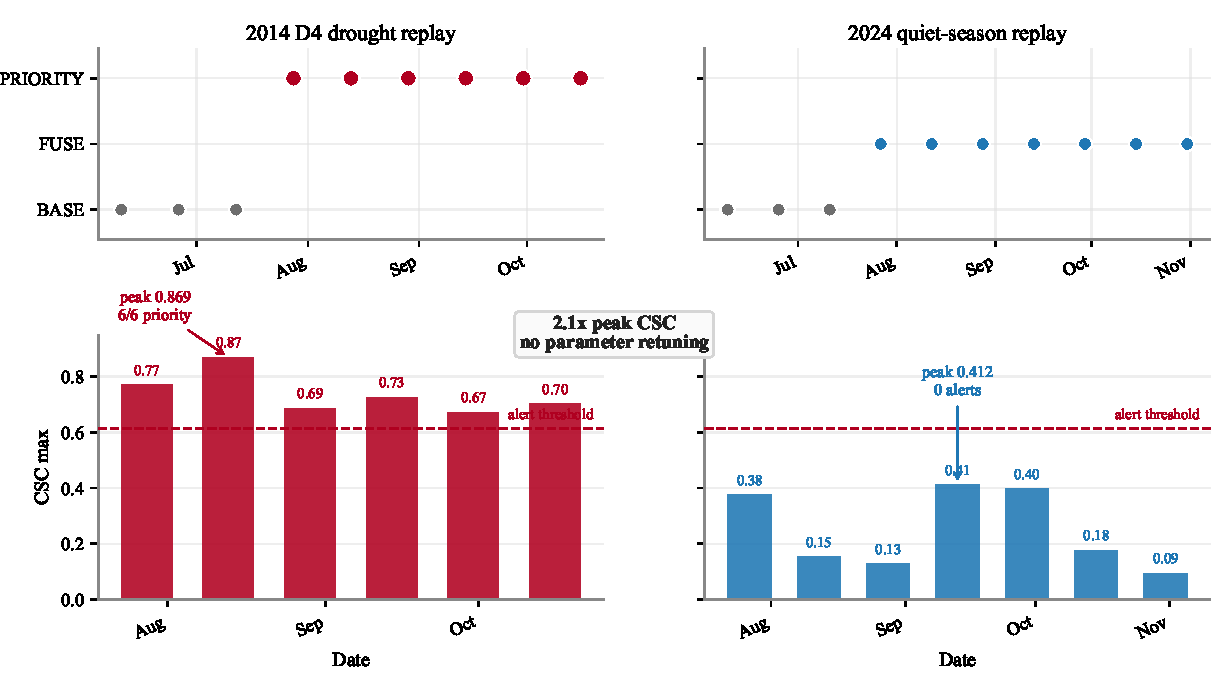
\includegraphics[width=\linewidth]{../figures/Figure_2_westlands_replay.pdf}
\caption{Westlands replay with unchanged policy parameters. \texttt{MOD13} denotes vegetation-only screening, \texttt{FUSE} denotes full CSC generation, and \texttt{FUSE\_PRIORITY} denotes fused alert tiles during downlink windows. The 2014 D4 drought season triggers priority alerts in every active post-warmup window, while the 2024 quiet season remains below the calibrated CSC alert threshold of 0.615.}
\label{fig:timeline}
\end{figure}

\begin{figure}[!h]
\centering
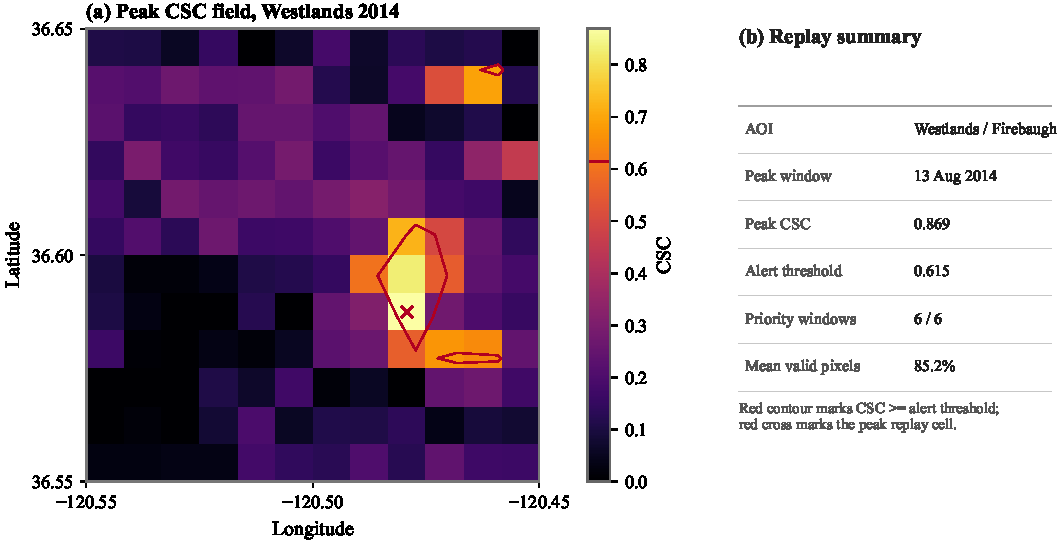
\includegraphics[width=\linewidth]{../figures/Figure_3_peak_alert_map.pdf}
\caption{Peak 2014 alert map generated from the tracked replay artifact. Pale cells, if present, indicate invalid or masked MODIS pixels. The red cross marks the peak grid-cell center at $36.587500^\circ$N, $120.479167^\circ$W; it is not a surveyed field point.}
\label{fig:alert-map}
\end{figure}

For live operation, users can run \texttt{real\_modis\_replay.py} with Earthdata credentials and an AppEEARS-accessible area of interest. To test another agricultural region, they can pass a new bounding box or area label through the replay command and keep the same policy thresholds. To test another onboard policy, they can subclass or replace \path{CASCADEPolicy}, then compare the regenerated action distribution, downlink volume, and alert windows against the accepted fixtures. The live path writes fresh outputs to \texttt{build/replay/}, keeping externally dependent downloads separate from the default offline review workflow.

\section{Impact}

CASCADE enables reusable experiments in onboard anomaly triage. The drought CSC used here is one instantiation of a broader interface: users provide a bounded stress or risk field, retain the same belief gate and action table, and compare policy outputs against common resource metrics. This supports new research questions about how much posterior evidence is enough to justify high-resolution confirmation, how energy and downlink constraints change sensing cadence, and how synthetic calibration behaves on historical scenes.

\begin{verbatim}
policy = CASCADEPolicy(csc_alert_thr=0.62)
risk = fire_risk_index(scene.ndvi, scene.lst, scene.moisture)
state = State(..., evi_anom=ndvi_loss,
              ndwi_anom=moisture_loss, csc=risk)
action = policy.act(state)
priority = policy.should_priority_downlink(state, risk)
\end{verbatim}

The package also improves existing remote-sensing questions. Many drought and crop-stress studies assume that imagery has already reached the ground. CASCADE lets researchers include the spacecraft decision layer in the experiment. The strongest concrete result is the synthetic 100-seed Monte Carlo benchmark: full CASCADE reduces downlink by 99.05\% versus raw collection, saves 38.3\% energy, preserves 100.0\% synthetic anomaly-event recall, and holds a 0.6\% false-positive rate. Against a fixed onboard baseline it reduces downlink by 77.6\% and energy by 25.4\%. These values are protected by validation tests and accepted fixtures, so changes to the scheduler or CSC calibration must either preserve them or update the evidence trail.

\begin{figure}[!h]
\centering
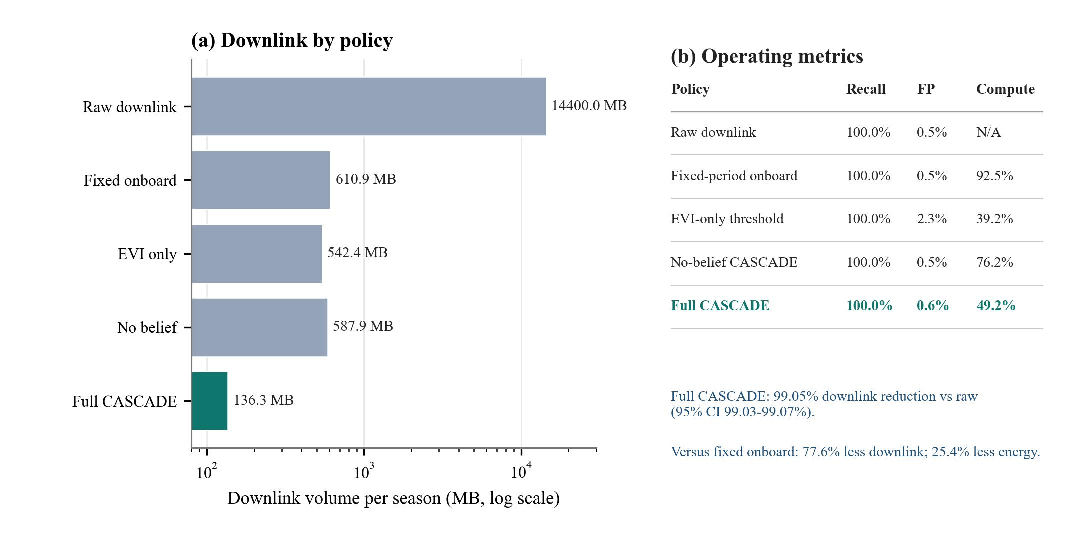
\includegraphics[width=\linewidth]{../figures/Figure_4_baseline_comparison.pdf}
\caption{Synthetic 100-seed Monte Carlo baseline comparison. Full CASCADE reduces downlink by 99.05\% versus raw collection and 77.6\% versus fixed-period onboard processing, while preserving 100.0\% synthetic anomaly-event recall at a 0.6\% false-positive rate.}
\label{fig:baseline-comparison}
\end{figure}

The Westlands replay is not a labeled anomaly-recall benchmark; it is an archival real-scene check that the same committed policy separates a known drought year from a quiet season. The 2014 California exceptional drought replay reaches peak CSC 0.869 and issues six priority alerts across six active post-warmup windows. The 2024 quiet-season replay peaks at CSC 0.412 and issues no priority alerts. Both runs use the same calibrated 0.615 alert threshold and the same tracked code path, providing a reproducible bridge between synthetic calibration and historical evidence of the 2012--2014 California drought \cite{griffin-anchukaitis-2014}.

Daily practice impact is currently prospective because CASCADE is pre-flight research software, not an operational advisory service. Its chosen lane is as a reference implementation for the NASA Space-to-Soil challenge community and as a pre-flight testbed for mission designers preparing hardware-in-the-loop or hosted-payload experiments. The package changes that workflow by replacing spreadsheet-level resource assumptions with executable replay, fixtures, and CI, giving future users a stable baseline before deployed uptake or commercial adoption can be measured.

\section{Conclusions}

CASCADE provides an executable, tested package for studying onboard Bayesian triage of crop stress from Earth observations. Its contribution is the integration of a CSC anomaly score, Beta-posterior belief gate, resource-aware action policy, simulation benchmark, and MODIS replay harness in a single open-source repository. The current release reproduces the Westlands drought/quiet-season separation and protects paper-facing metrics through CI and accepted artifacts. Future work will extend the replay set beyond Westlands, run hardware-in-the-loop tests on flight-like processors, and generalize the anomaly-index interface to additional environmental monitoring domains.

\section*{Funding}

This research did not receive any specific grant from funding agencies in the public, commercial, or not-for-profit sectors.

\section*{Declaration of competing interest}

The author declares no known competing financial interests or personal relationships that could have appeared to influence the work reported in this paper.

\section*{Data availability}

The source code, validation fixtures, and release artifacts are available at \url{https://github.com/emillambert/CASCADE}. The SoftwareX code metadata table points to the intended v1.0.0 GitHub release. Live MODIS replay depends on NASA AppEEARS and Earthdata credentials; offline replay artifacts needed for the illustrative examples are included in the repository.

\section*{Declaration of generative AI and AI-assisted technologies in the manuscript preparation process}

During manuscript preparation, the author used OpenAI ChatGPT/Codex for planning, repository inspection, wording suggestions, and LaTeX drafting assistance. The author reviewed and edited the manuscript, verified the software outputs, and remains responsible for all scientific claims, citations, and submission materials. No scientific data or benchmark results were generated by AI tools.

\bibliographystyle{elsarticle-num}
\bibliography{../references}

\section*{Current executable software version}

CASCADE is a pure-Python package. The executable software version is the same as the source-code release listed in Table 1: v1.0.0 at \url{https://github.com/emillambert/CASCADE/releases/tag/v1.0.0}. There is no separate compiled binary artifact.

\end{document}
